\documentclass[12pt, spanish]{article}
\usepackage[spanish]{babel}
\selectlanguage{spanish}
%\usepackage{natbib}
\usepackage{url}
\usepackage[utf8x]{inputenc}
\usepackage{graphicx}
\graphicspath{{images/}}
\usepackage{parskip}
\usepackage{fancyhdr}
\usepackage{vmargin}

\usepackage{minted}
\usemintedstyle{vim}

\usepackage{hyperref}
\usepackage[
    type={CC},
    modifier={by-nc-sa},
    version={4.0},
]{doclicense}

\hypersetup{
    colorlinks=true,
    linkcolor=blue,
    filecolor=magenta,      
    urlcolor=cyan,
}

\usepackage[default]{sourcesanspro}

\usepackage[nottoc]{tocbibind}

\setmarginsrb{2 cm}{1 cm}{2 cm}{2 cm}{1 cm}{1.5 cm}{1 cm}{1.5 cm}

\title{Ingeniería de Servidores:\\
Práctica 3. \hspace{0.05cm} }                           
\author{Antonio David Villegas Yeguas}                             
\date{\today}                                           

\renewcommand*\contentsname{hola}

\makeatletter
\let\thetitle\@title
\let\theauthor\@author
\let\thedate\@date
\makeatother

\pagestyle{fancy}
\fancyhf{}
\rhead{\theauthor}
\lhead{\thetitle}
\cfoot{\thepage}

\begin{document}
%%%%%%%%%%%%%%%%%%%%%%%%%%%%%%%%%%%%%%%%%%%%%%%%%%%%%%%%%%%%%%%%%%%%%%%%%%%%%%%%%%%%%%%%%

\begin{titlepage}
    \centering
    \vspace*{0.5 cm}
    
\includegraphics[scale = 0.50]{ugr.png}\\[1.0 cm]
    %\textsc{\LARGE Universidad de Granada}\\[2.0 cm]   
    \textsc{\large 3ºA - A2}\\[0.5 cm]            
    \textsc{\large Grado en Ingeniería Informática}\\[0.5 cm]              
    \rule{\linewidth}{0.2 mm} \\[0.2 cm]
    { \huge \bfseries \thetitle}\\
    \rule{\linewidth}{0.2 mm} \\[1 cm]
    
    \begin{minipage}{0.4\textwidth}
        \begin{flushleft} \large
            \emph{Autor:}\\
            \theauthor
            \end{flushleft}
            \end{minipage}~
            \begin{minipage}{0.4\textwidth}
            \begin{flushright} \large
            \emph{Asignatura: \\
            Ingeniería de Servidores}                   
        \end{flushright}
    \end{minipage}\\[0.5cm]
  
    {\large \thedate}\\[0.5cm]
    {\url{https://github.com/advy99/ISE/}}
    {\doclicenseThis}
 	
    \vfill
    
\end{titlepage}

%%%%%%%%%%%%%%%%%%%%%%%%%%%%%%%%%%%%%%%%%%%%%%%%%%%%%%%%%%%%%%%%%%%%%%%%%%%%%%%%%%%%%%%%%

\tableofcontents
\pagebreak

%%%%%%%%%%%%%%%%%%%%%%%%%%%%%%%%%%%%%%%%%%%%%%%%%%%%%%%%%%%%%%%%%%%%%%%%%%%%%%%%%%%%%%%%%



\section{Instalación de Zabbix}


Tras configurar el nuevo disco en el RAID1 y monitorizar los discos disponibles en nuestro RAID1 con systemd, llegamos al punto de la instalación de Zabbix.

Para esto, primero es conveniente leer el manual de Zabbix\cite{zabbix_man} dado en el guión de prácticas de esta práctica.

Tras leer la introducción del manual, en la que nos explican la estructura del manual y una breve descripción de cada apartado así como los distintos softwares que tiene Zabbix (cliente, servidor, proxy, etc) , pasamos a la instalación.

En nuestro caso, instalaremos Zabbix Server en Ubuntu y Zabbix Agent en Ubuntu y CentOS,  así que nos centraremos en estos SO, cabe decir el manual de Zabbix contempla la instalación del software para Ubuntu, RHEL/CentOS y cualquier distribución a través del código fuente, ya que Zabbix es libre.

\subsection{Instalación en Ubuntu}

Lo primero que encontramos en el manual de instalación son las formas de obtener Zabbix, que son las siguientes:

\begin{enumerate}
	\item{Desde el código fuente}
	\item{Desde paquetes precompilados}
\end{enumerate}

En nuestro caso, utilizaremos la instalación desde paquetes precompilados para que APT se encargue de resolver los problemas de dependencias y requisitos al instalar Zabbix.

Lo instalamos de la siguiente forma:

\begin{minted}[linenos,tabsize=2,breaklines]{bash}
# wget https://repo.zabbix.com/zabbix/3.4/ubuntu/pool/main/z/zabbix-release/\
zabbix-release_3.4-1+xenial_all.deb
# dpkg -i zabbix-release_3.4-1+xenial_all.deb
# apt update
\end{minted}

\newpage

Vemos como se ha instalado correctamente:
\begin{center}
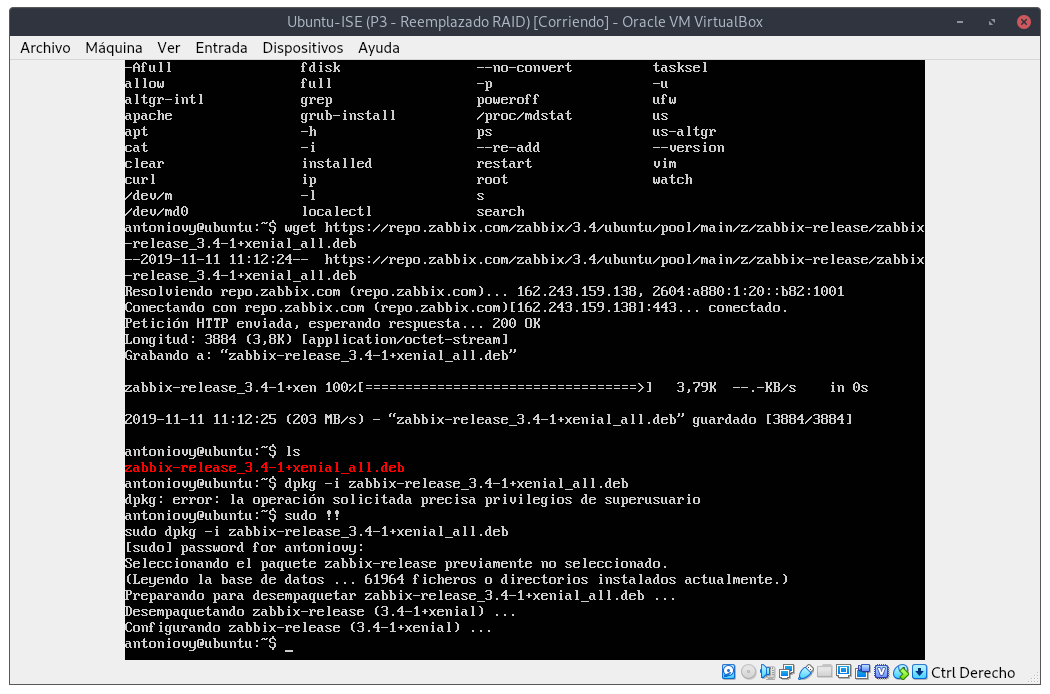
\includegraphics[scale=0.45]{instalacion_zabbix.png}
\end{center}

Aun así esto solo ha instalado los repositorios de Zabbix en Ubuntu, ahora pasamos a instalar el servidor de Zabbix con MySQL, el frontend de Zabbix Server y el cliente de Zabbix:

\vspace{2cm}

\begin{minted}[linenos,tabsize=2,breaklines]{bash}
# apt install zabbix-server-mysql
# apt install zabbix-frontend-php
# apt install zabbix-agent
\end{minted}

\vspace{2cm}

Y con esto, tenemos el servidor y cliente de Zabbix instalado, pasamos a la configuración.

\newpage

Por último, comentar un detalle bastante importante, el manual de Zabbix nos indica que para activar y habilitar Zabbix hay que utilizar el comando \texttt{service} y el sistema de servicio \texttt{update-rc}, sin embargo, como nos avisa la instalación, este software ya no esta en uso, ya que ha sido sustituido por SystemD, por este motivo yo usaré \texttt{systemctl} para gestionar los distintos procesos de Zabbix.


\begin{center}
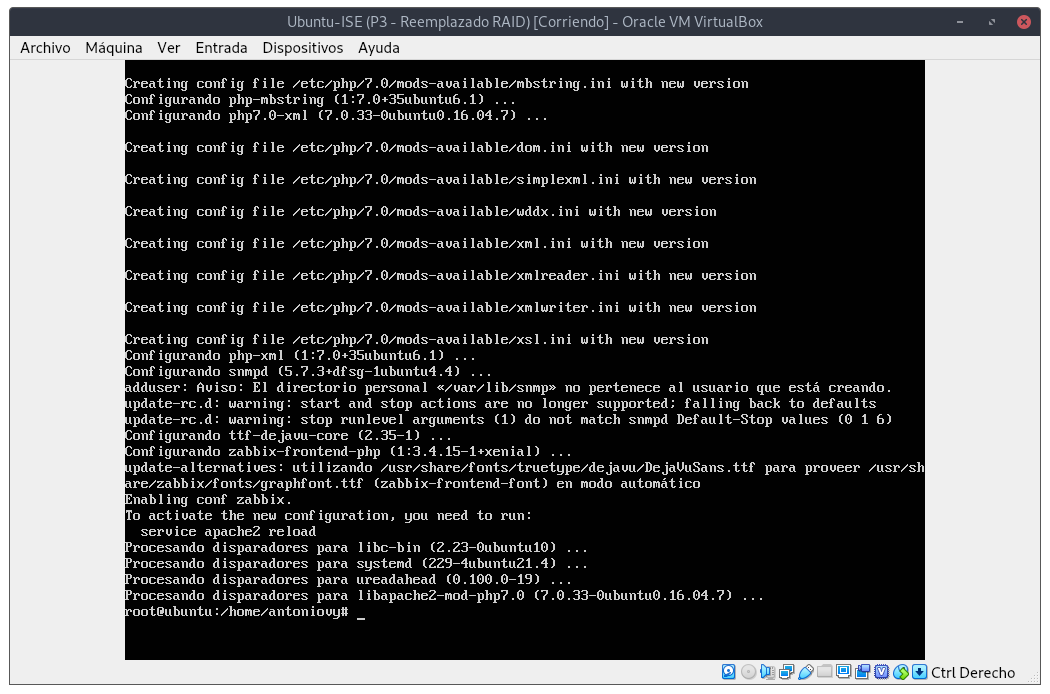
\includegraphics[scale=0.45]{aviso_instalacion.png}
\end{center}


\subsection{Creación de la BD}

Una vez instalado Zabbix, es necesario crear una base de datos, para realizar este paso consultaremos el apendice del manual de Zabbix, en concreto la sección en la que nos enseñan a crear una BD\cite{zabbix_apendice_BD}.

El primer paso, como indican, es localizar los archivos \texttt{schema.sql, images.sql} y \texttt{data.sql}, que al instalarlo por lo paquetes, tenemos esos archivos en:

\texttt{/usr/share/doc/zabbix-server-mysql/create.sql.gz}, y solo será necesario realizar los primeros pasos de la creación de la BD, ya que los siguientes están en la instalación específica de Ubuntu.


\begin{minted}[linenos,tabsize=2,breaklines]{mysql}
shell> mysql -u root -p
mysql> create database zabbix character set utf8 collate utf8_bin;
mysql> grant all privileges on zabbix.* to zabbix@localhost identified by '<password>';
mysql> quit;
\end{minted}



Donde para nosotros, \texttt{<password>} será \texttt{practicas,ISE}

\begin{center}
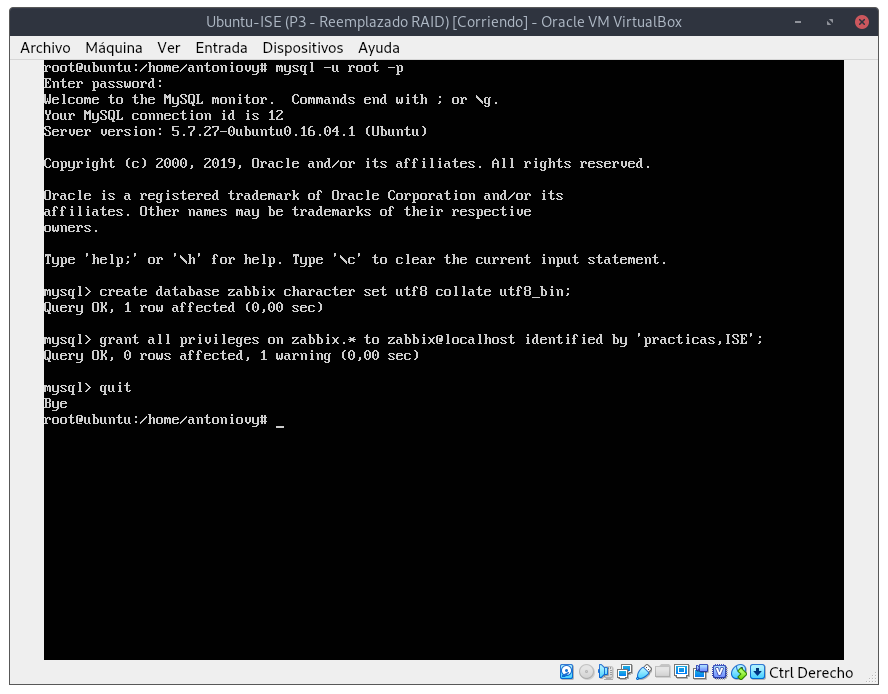
\includegraphics[scale=0.45]{creacion_BD.png}
\end{center}

Y pasamos a exportar el esquema inicial de la base de datos:

\begin{minted}[linenos,tabsize=2,breaklines]{bash}
# zcat /usr/share/doc/zabbix-server-mysql/create.sql.gz | mysql -u zabbix -p zabbix
\end{minted}

Podemos comprobar que se ha realizado correctamente entrando en MySQL y comprobando las tablas de la BD zabbix:

\begin{minted}[linenos,tabsize=2,breaklines]{mysql}
shell> mysql -u zabbix -p zabbix
mysql> show tables;
mysql> quit;
\end{minted}

\newpage

\subsection{Configuración de Zabbix Server}

Ahora pasamos a la configuración del servidor de Zabbix, para esto pasamos a editar el archivo de configuración, ubicado en \texttt{/etc/zabbix/zabbix\_server.conf}

\begin{minted}[linenos,tabsize=2,breaklines]{bash}
# vi /etc/zabbix/zabbix_server.conf
DBHost=localhost
DBName=zabbix
DBUser=zabbix
DBPassword=practicas,ISE 
\end{minted}

Es necesario establecer \texttt{DBHost} a \texttt{localhost}, para que use MySQL y no PostgreSQL y establecar \texttt{DBPassword} a \texttt{practicas,ISE}, mientras que DBName y DBUser ya vienen con esos valores por defecto.


Por último, activamos y habilitamos el servicio de zabbix:
\begin{minted}[linenos,tabsize=2,breaklines]{bash}
# systemctl start zabbix-server
# systemctl enable zabbix-server
\end{minted}

Un detalle importante, es que aunque actualmente estemos en Ubuntu, pero si el servidor lo instalamos en CentOS debemos activar las distintas flags de SELinux para permitir que un servicio http se conecte a las bases de datos.



\subsection{Configuración del front-end}

La configuración del cliente de Zabbix la podemos encontrar en:

\texttt{/etc/apache2/conf-enabled/zabbix.conf}

La configuración ya está activada, sin embargo hay que quitar el comentario de la linea con el valor para la zona horaria.


Por último, reiniciamos apache2:
\begin{minted}[linenos,tabsize=2,breaklines]{bash}
# systemctl restart apache2
\end{minted}

\subsection{Configuración de Zabbix Agent en Ubuntu}

Ubuntu al tener instalado el servidor en el mismo sistema operativo no necesita configurar zabbix-agent, con iniciar el proceso basta, además de añadir en ufw el puerto usado por Zabbix, el 10050. Esto último no es obligatorio ya que se va a conectar con la propia máquina, pero en caso de tener el servidor Zabbix instalado en otra máquina si es necesario.
\begin{minted}[linenos,tabsize=2,breaklines]{bash}
# systemctl start zabbix-agent
# systemctl enable zabbix-agent
# ufw allow 10050
\end{minted}



\subsection{Configuración de Zabbix a través del navegador}

Con todo esto, ya tenemos Zabbix disponible en el navegador y pasamos a su configuración:

\subsubsection{Configuración inicial:}

\begin{center}
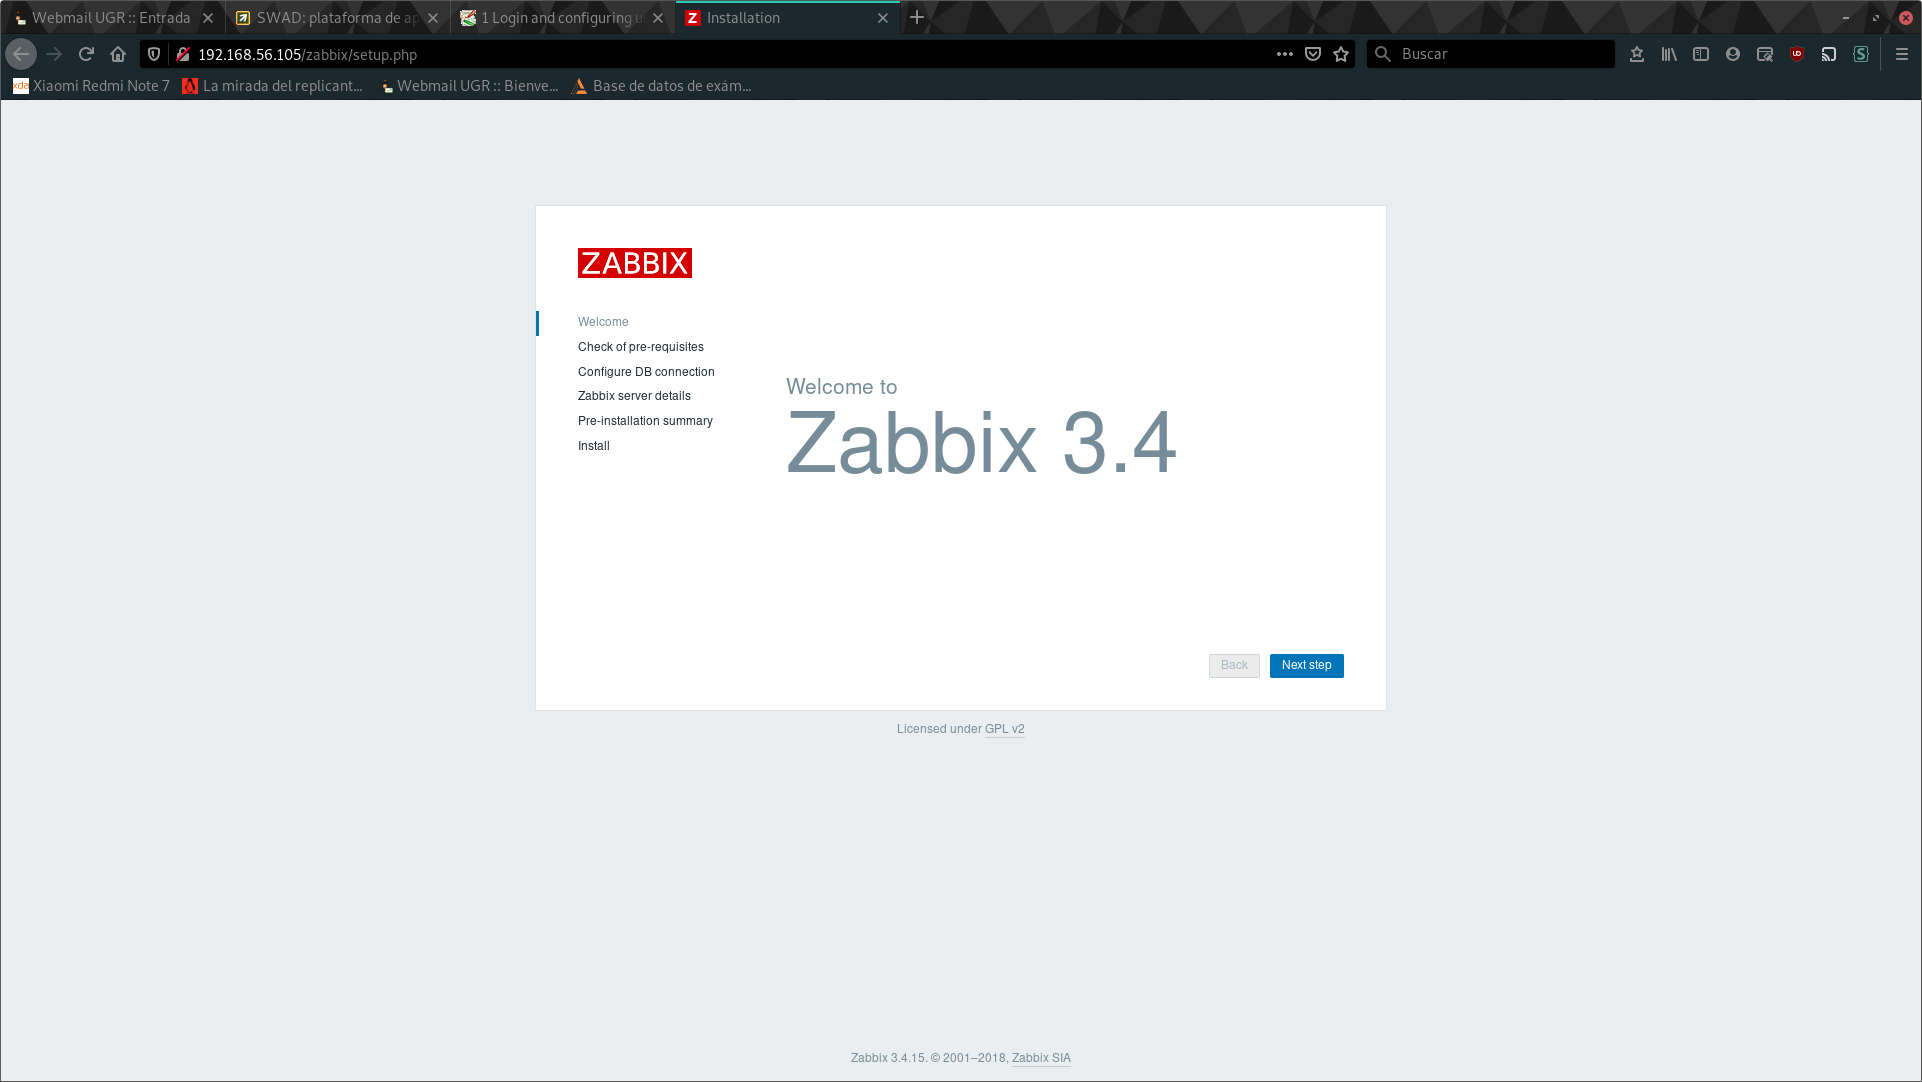
\includegraphics[scale=0.25]{zabbix_instalado.png}
\end{center}

En la siguiente pestaña veremos como todos los paquetes necesarios son correctos, y en la siguiente nos pedirá conectarnos a la base de datos creada para Zabbix, cuya configuración es la por defecto, añadiendo la clave usada, es decir, \texttt{practicas,ISE}, manteniendo el host en \texttt{localhost}, y el nombre de la BD y el nombre de usuario en \texttt{zabbix}.

\newpage

Ahora pasamos a poner el host e IP del servidor de Zabbix, los cuales dejaremos por defecto, además de el nombre de la instalación, que en mi caso pondré Zabbix-Server19, y con esto acabamos la configuración inicial:

\begin{center}
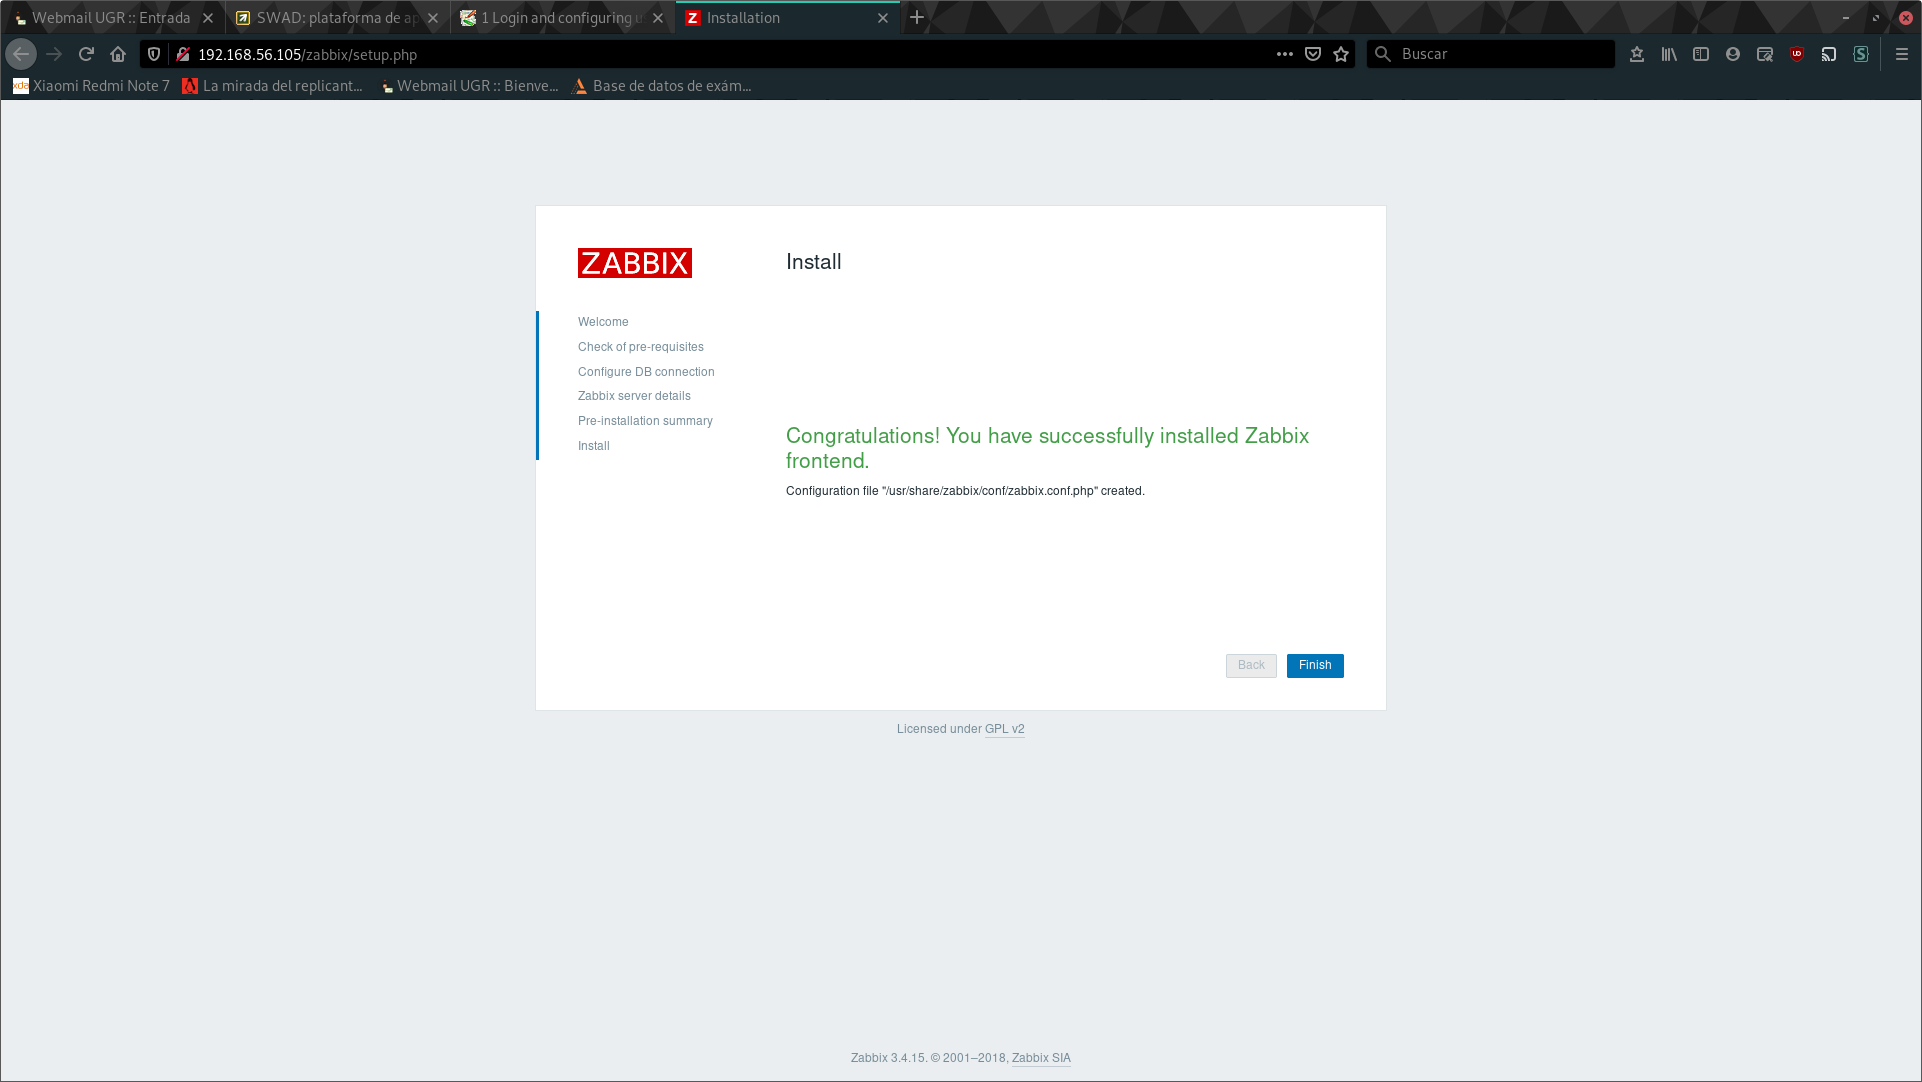
\includegraphics[scale=0.25]{instalacion_acabada.png}
\end{center}



\subsubsection{Crear un usuario:}
Con esto podremos acceder a Zabbix a través del navegador usando el usuario \texttt{Admin} y contraseña \texttt{zabbix}. Lo primero que haremos será cambiar este usuario y contraseña como nos explican en su manual de configuración rápida\cite{zabbix_quickstart}, en concreto en el menú Administración -> Usuarios, desde este menú podremos gestionar todos los usuarios de Zabbix. Vemos como por defecto existen dos usuarios, el administrador y el invitado. 


\subsubsection{Gestionar permisos:}

En mi caso, crearé un usuario con permisos de lectura a Linux servers para que sea capaz de monitorizar el sistema.

En el caso de Zabbix, los permisos se gestionan por grupos, es decir, nosotros no asignaremos los permisos a un usuario, si no a un grupo, así que para que un usuario tenga ciertos permisos (asociados a un grupo) este usuario debe pertenecer al grupo que tenga esos permisos.

\begin{center}
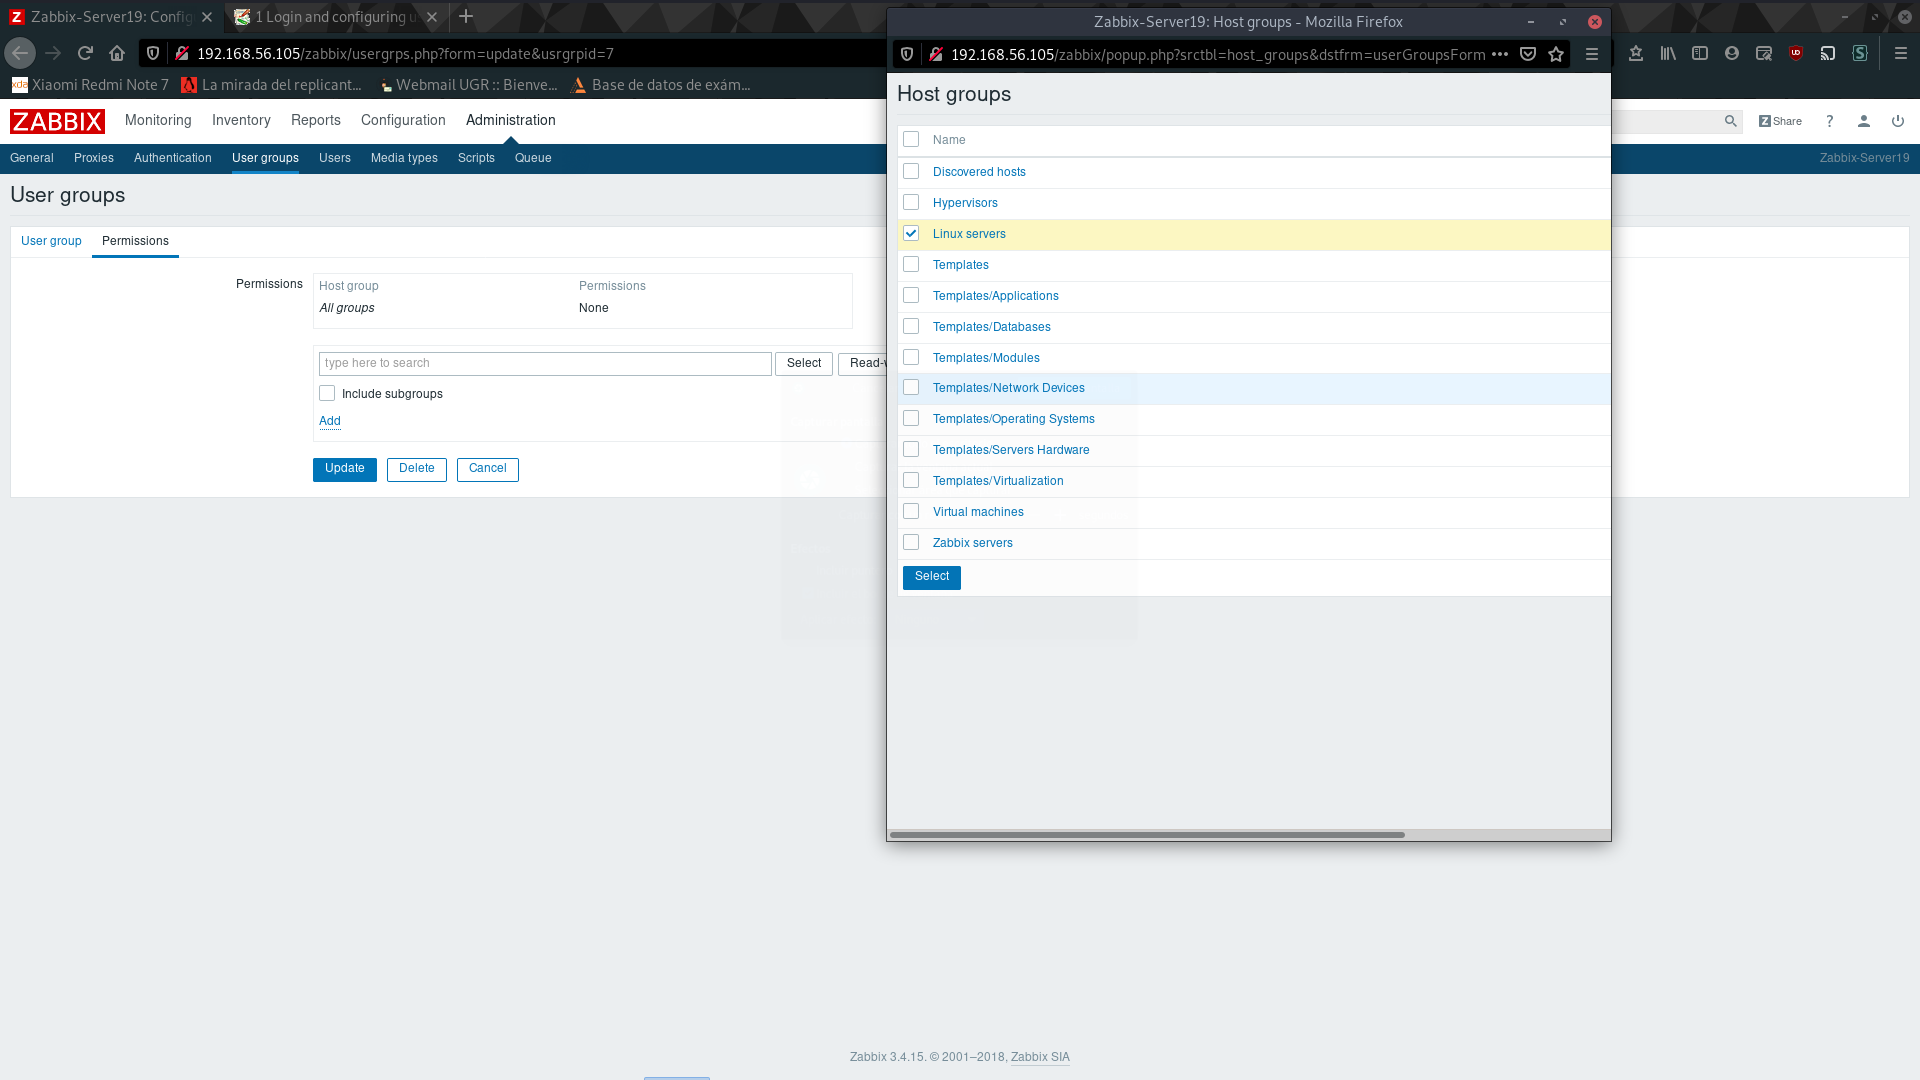
\includegraphics[scale=0.25]{permisos_zabbix.png}
\end{center}



\section{Configurar Zabbix Agent en CentOS}

\subsection{Instalación de zabbix-agent}
Para monitorizar CentOS lo primero que tenemos que hacer es instalar \texttt{zabbix-agent} y permitir el puerto que usaremos para conectarnos al servidor:

\begin{minted}[linenos,tabsize=2,breaklines]{bash}
# rpm -ivh https://repo.zabbix.com/zabbix/3.4/rhel/7/x86_64/zabbix-release-3.4-2.el7.noarch.rpm
# yum install zabbix-agent
# firewall-cmd --add-port=10050/tcp
# firewall-cmd --add-port=10050/tcp --permanent
\end{minted}

\subsection{Configuración del agente}
Una vez instalado, modificamos el archivo de configuración \texttt{/etc/zabbix/zabbix\_agentd.conf} y establecemos el Server a 192.168.56.105, que es donde se encuentra el servidor de Zabbix
\begin{center}
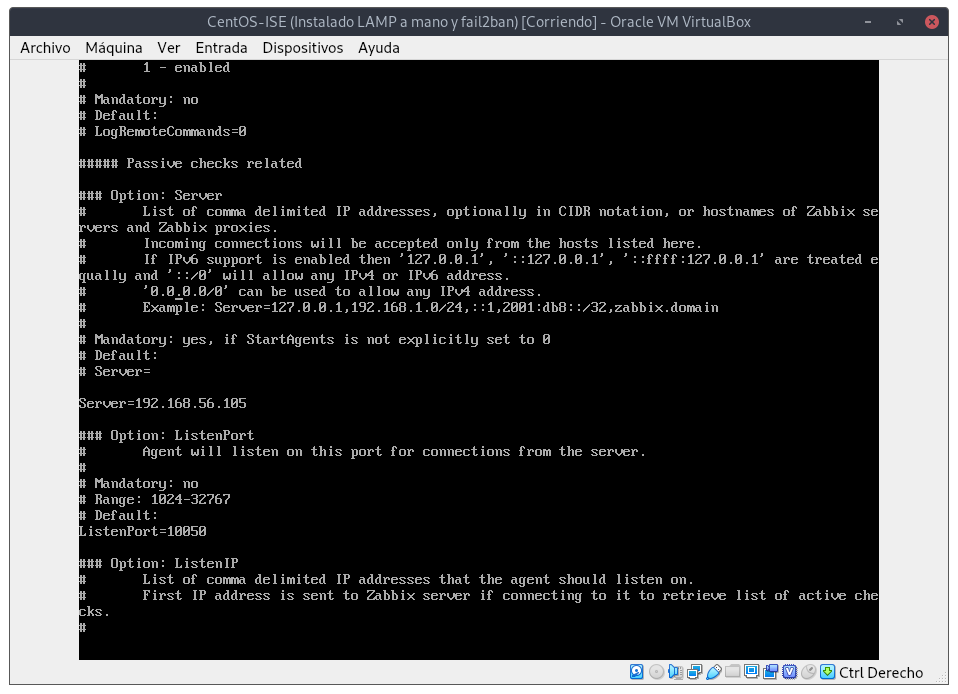
\includegraphics[scale=0.25]{centos_conf.png}
\end{center}


Pasamos a activar el servicio
\begin{minted}[linenos,tabsize=2,breaklines]{bash}
# systemctl start zabbix-agent
\end{minted}


Sin embargo, vemos que falla, y \texttt{journalctl -xe} junto con \texttt{/var/log/audir/audit.log} nos damos cuenta de que el problema es SELinux, que no nos permite modificar el archivo de configuración
\begin{center}
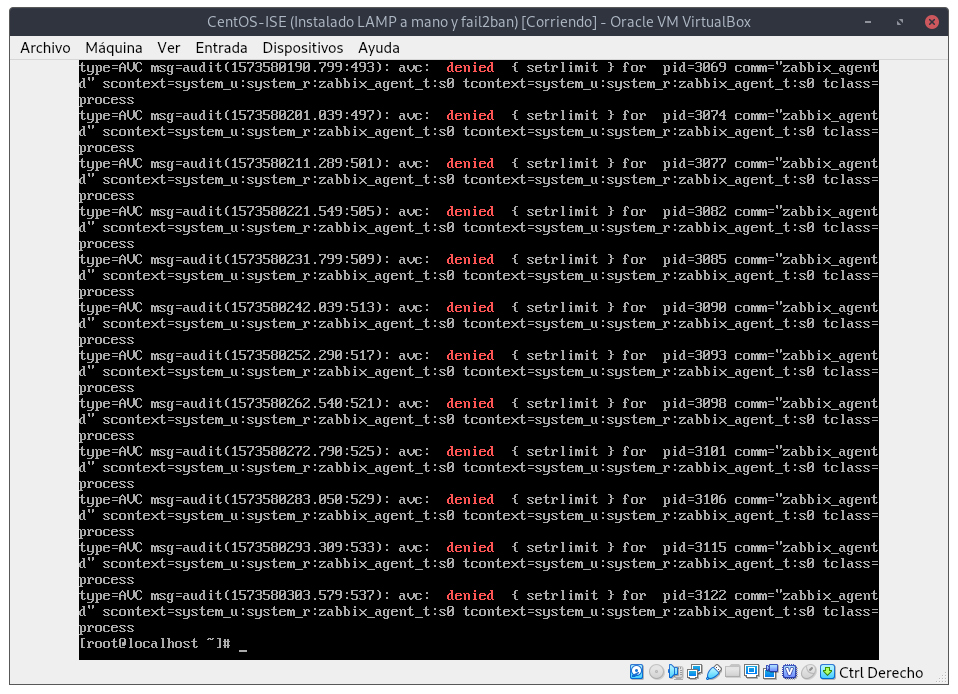
\includegraphics[scale=0.25]{selinux.png}
\end{center}

Este es un problema común que no encontraremos en el manual, pero rápidamente podemos encontrar la solución en los foros de Zabbix\cite{zabbixSElinux}.

Para resolver este problema usaremos la herramienta \texttt{audit2allow}\cite{audit2allow_man}, que nos permite crear una política de SELinux a través del archivo \texttt{/var/log/audit/audit.log}
\begin{minted}[linenos,tabsize=2,breaklines]{bash}
# grep zabbix_agent_t /var/log/audit/audit.log | audit2allow -M zabbix_agentd_custom
# semodule -i zabbix_agentd_custom.pp
# systemctl restart zabbix-agent
\end{minted}

Y con esto, zabbix-agent ya esta activado y funcionando, como podemos ver usando \texttt{zabbix\_get}, podemos acceder desde Ubuntu.
\begin{center}
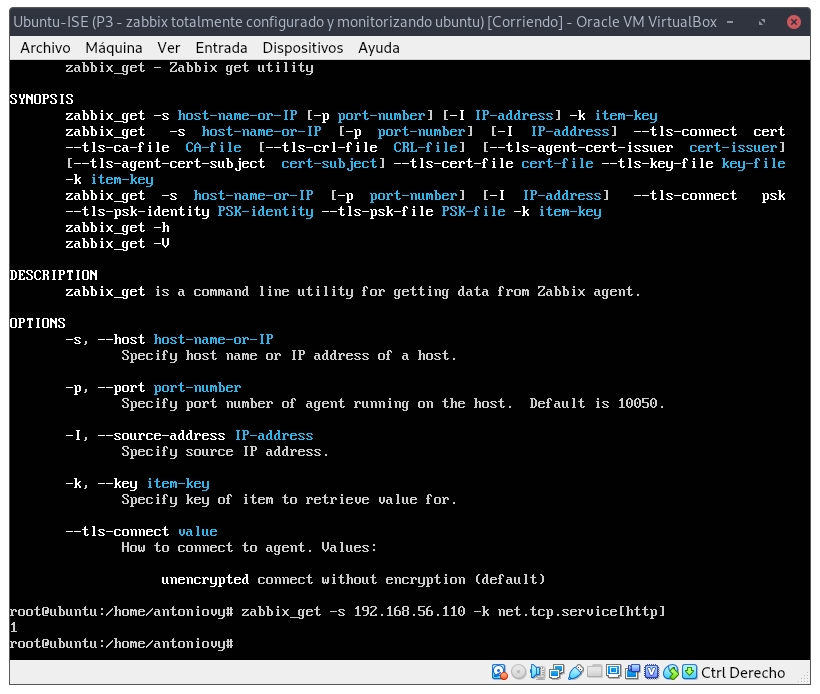
\includegraphics[scale=0.25]{zabbix_get.png}
\end{center}



\section{Monitorizar máquinas}

En esta sección se muestra contenido común a Ubuntu y CentOS, la única diferencia será la IP, que cuando estemos en el host de Ubuntu será \texttt{127.0.0.1}, es decir localhost, ya que se monitoriza a si mismo, mientras que para referirnos al host de CentOS usaremos \texttt{192.168.56.110}, ya que es la IP donde se encuentra CentOS en nuestra red.


\subsection{Añadir máquinas a monitorizar:}

Una vez tenemos configurado el nuevo usuario, pasamos a configurar el host, es decir, añadir en Zabbix la maquina que queremos monitorizar.

Por defecto, Zabbix nos añade la máquina en la que se ejecuta Zabbix, aunque su monitorización está desactivada por defecto. Yo dejare desactivado este y añadir uno nuevo aunque también tenga como host a \texttt{localhost}.

Para esto, desde la cuenta \texttt{Admin} añadimos un host en Administración -> Hosts.

Para crear un host indicamos el nombre que le queremos dar, la IP del host y el puerto (este último lo dejamos por defecto) y en Grupos añadimos Linux servers.


\subsection{Añadir items a una máquina:}

Ya tenemos la máquina añadida, ahora tenemos que decirle que partes del servidor queremos monitorizar.

Para esto, en la sección de host entramos en el nuevo host,  y en la sección items creamos un item con lo que queramos monitorizar.

Por ejemplo, crearemos un item para la carga de CPU, en key tenemos que buscar y poner \texttt{system.cpu.load} y crearemos una nueva aplicación a la que llamaremos \texttt{CPU} donde almacenaremos todos los items que traten sobre la CPU.

\begin{center}
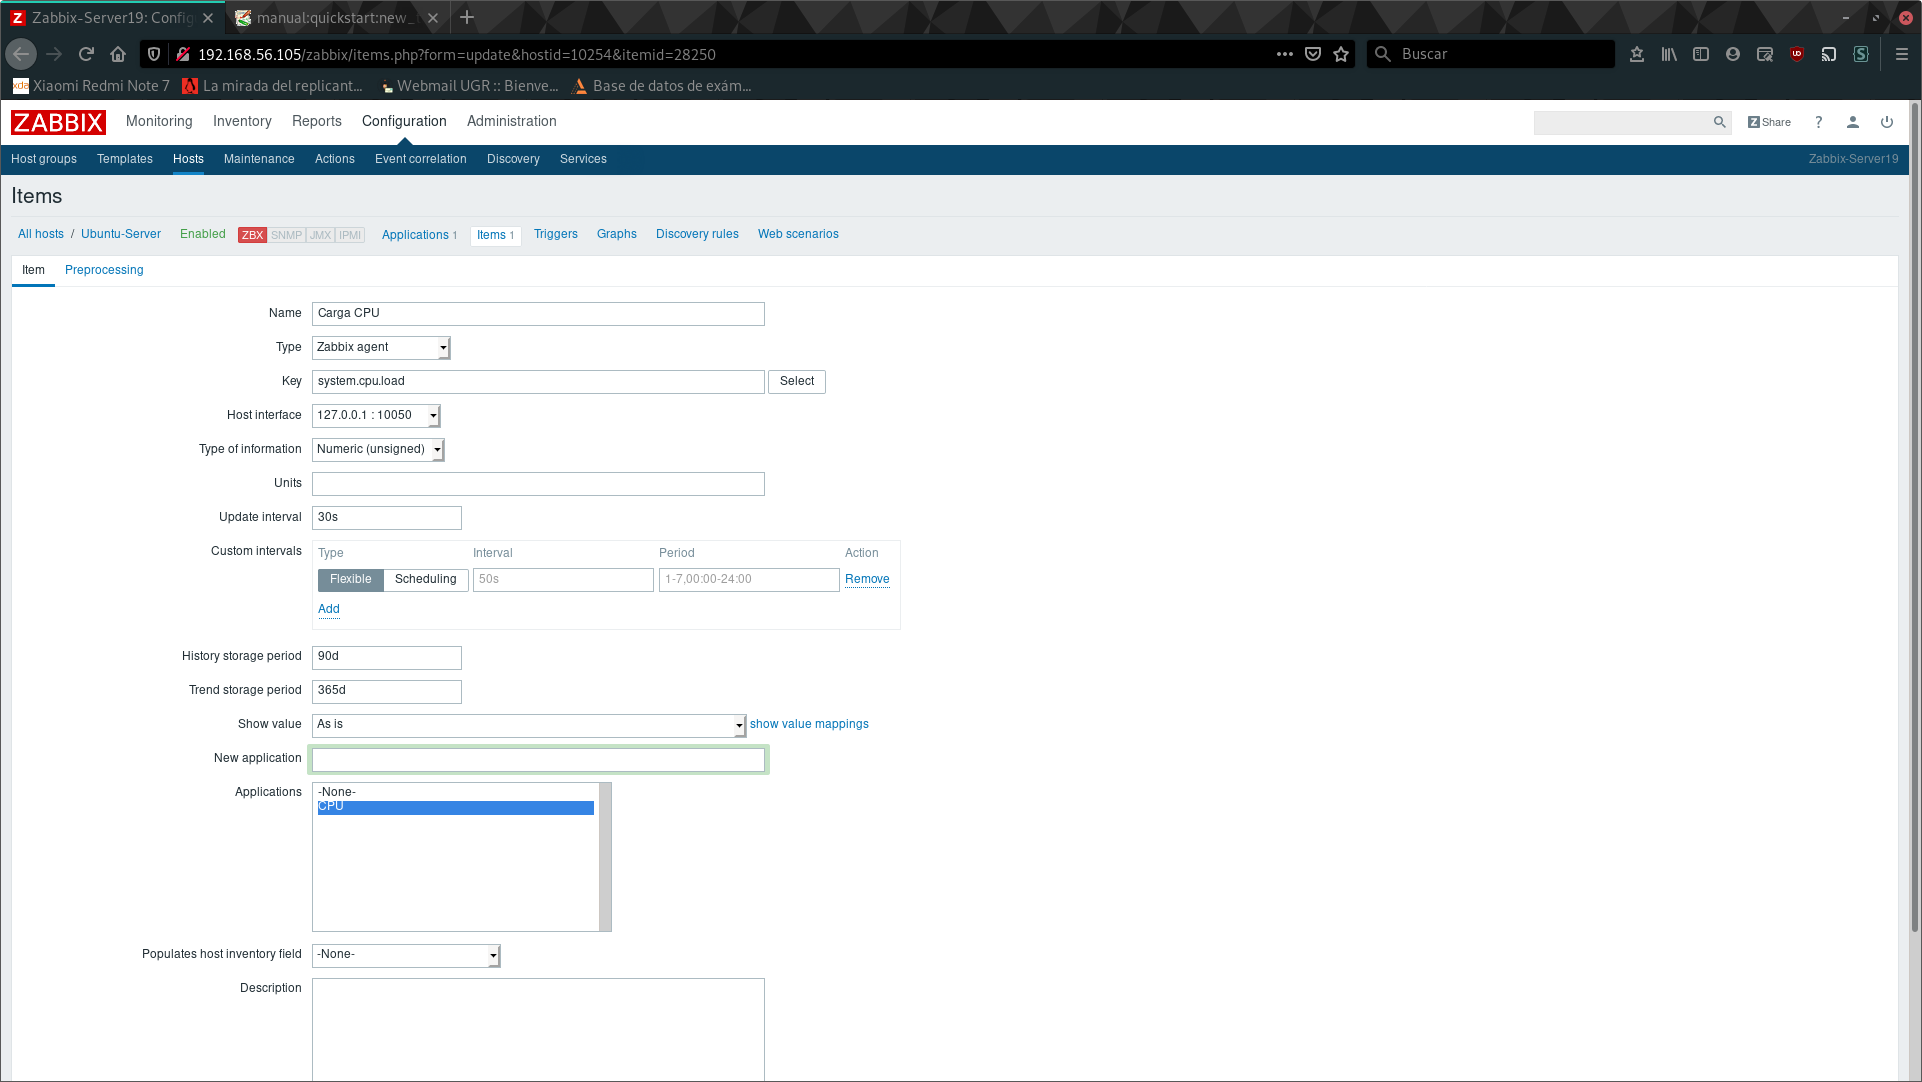
\includegraphics[scale=0.25]{item_zabbix.png}
\end{center}

\subsection{Revisar los datos}

Y con esto, ya vemos que vemos la carga de la CPU de Ubuntu en la sección Monitoring -> Latest data:

\begin{center}
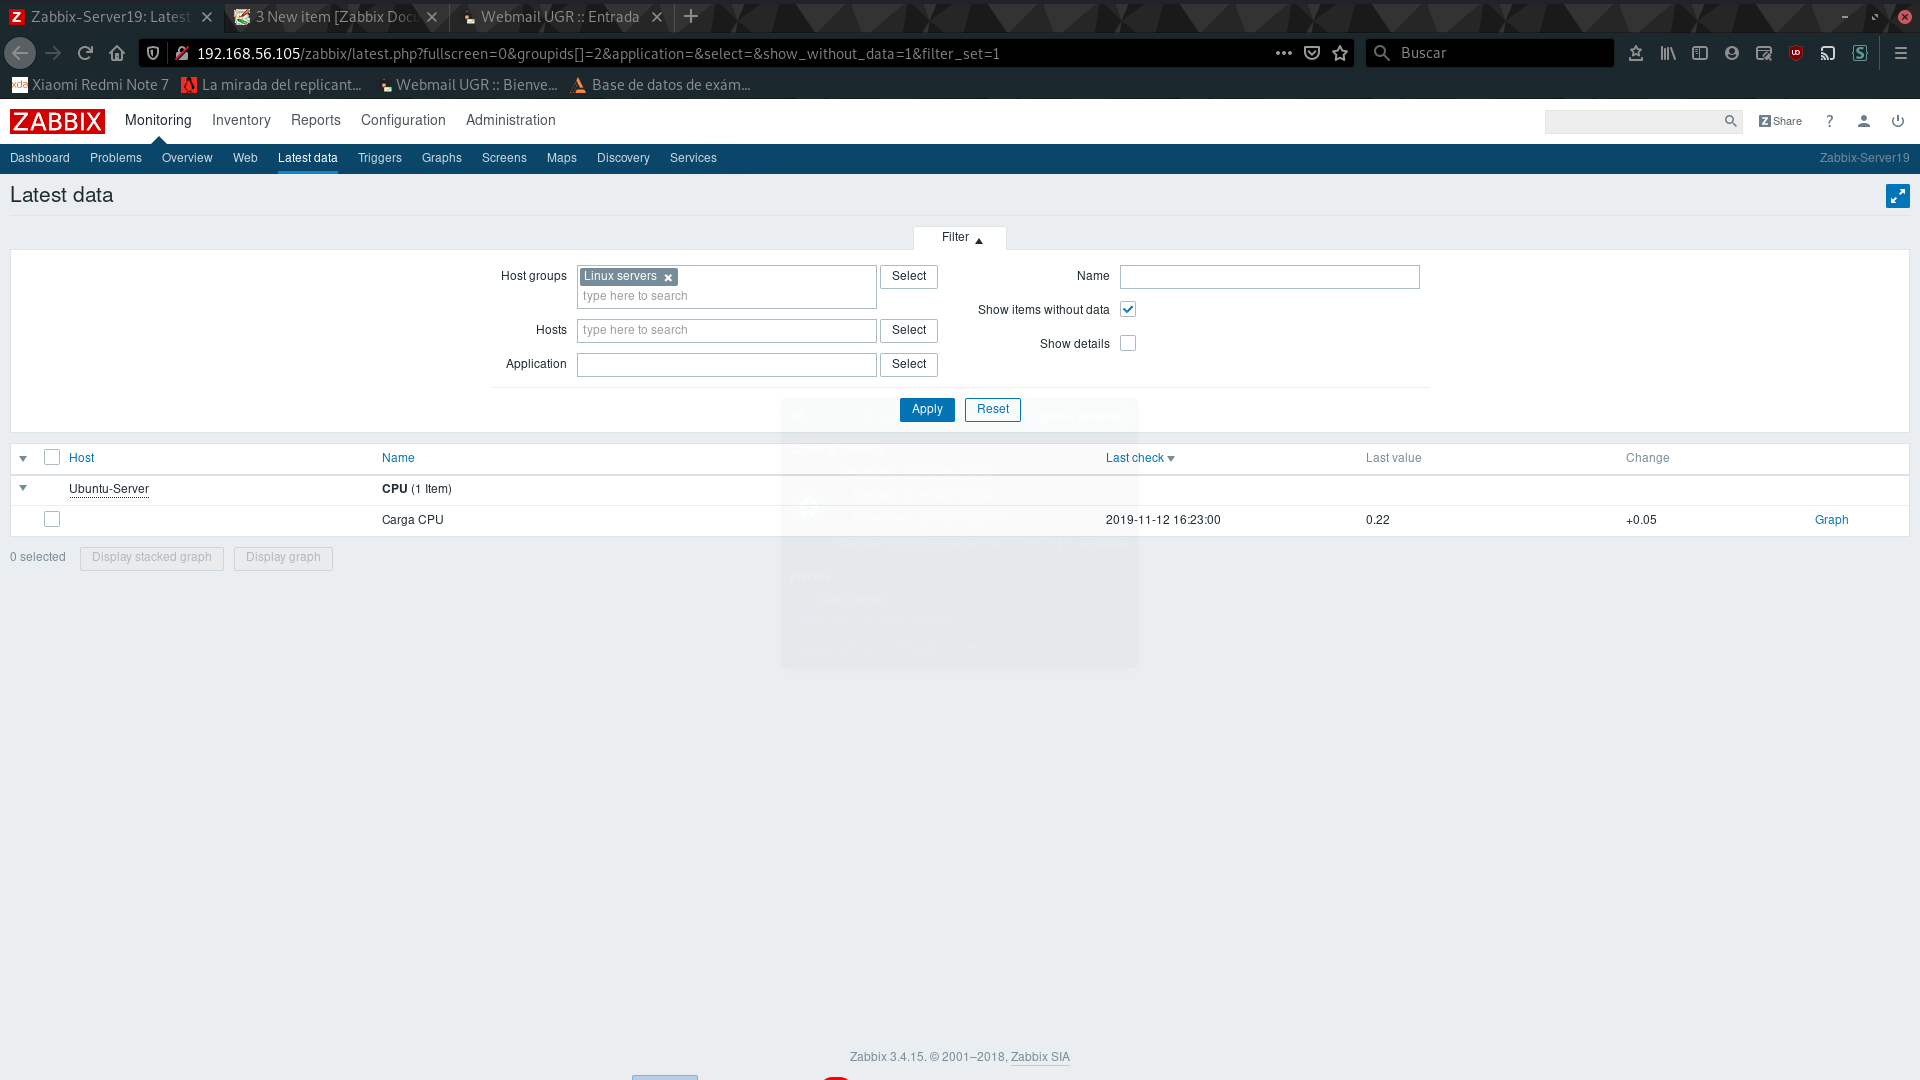
\includegraphics[scale=0.25]{item_1.png}
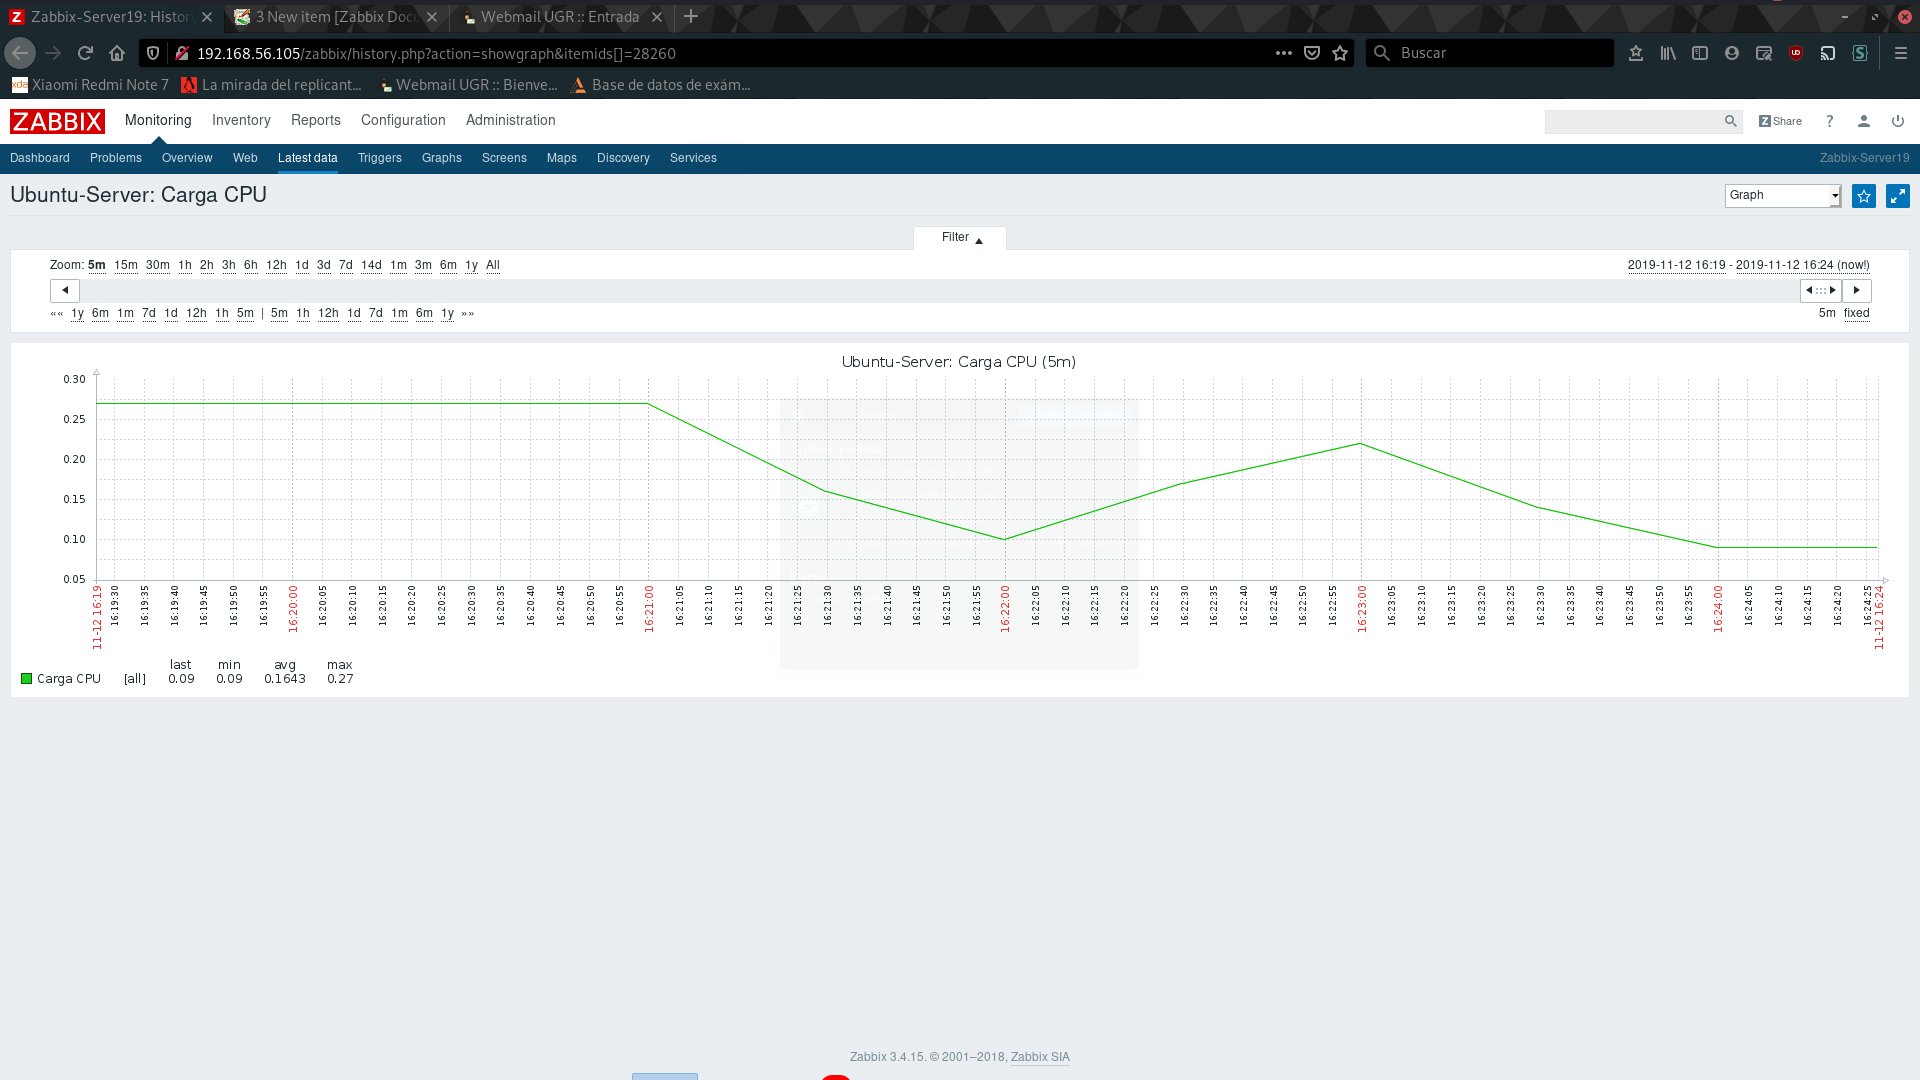
\includegraphics[scale=0.25]{item_2.png}
\end{center}

Yo además he añadido dos templates, una para monitorizar SSH y otra para el servidor HTTP, usando la sección templates.

\newpage

Vemos como HTTP no da ningun problema, sin embargo, SSH esta caído, esto se debe a que por defecto, el template de SSH tiene el puerto 22, y nosotros usamos el puerto 22022:
\begin{center}
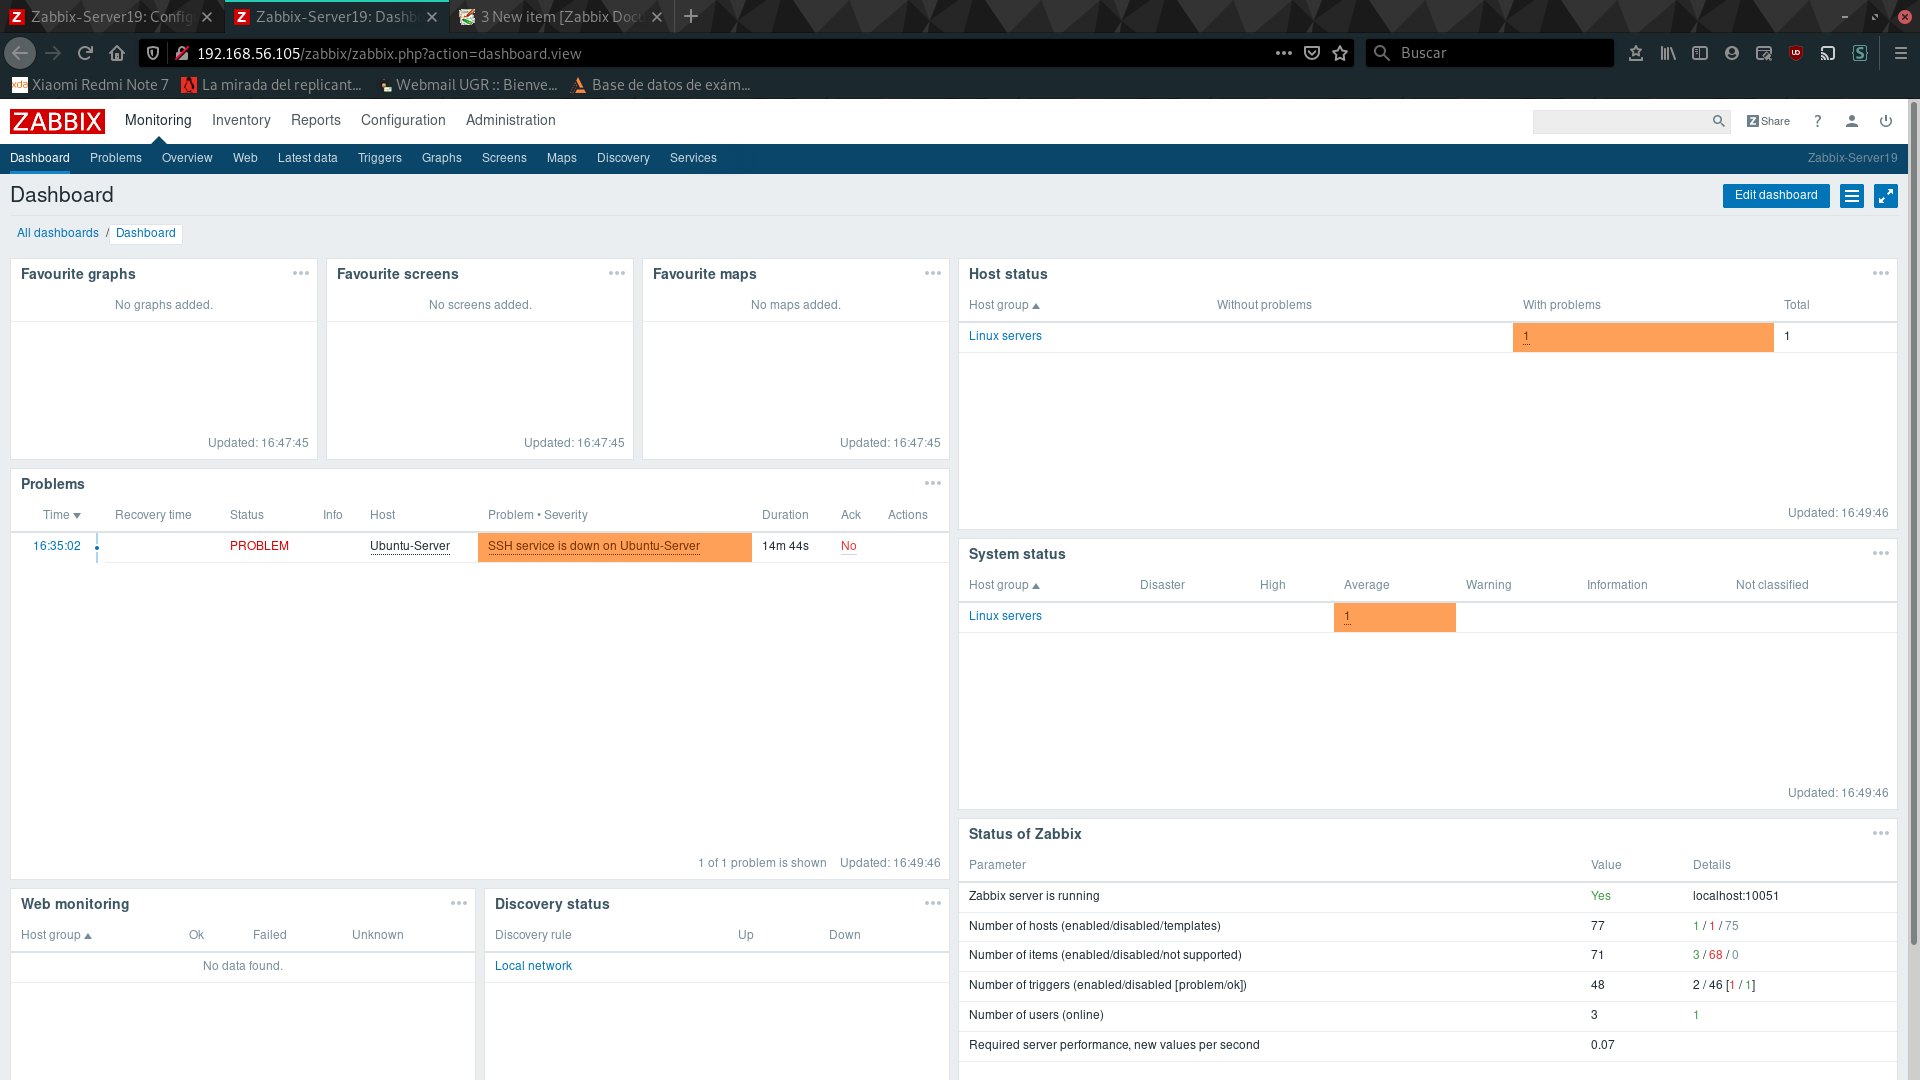
\includegraphics[scale=0.25]{error_ssh.png}
\end{center}

Eliminamos el template de SSH, y lo añadimos manualmente, usando la clave \\
\texttt{net.tcp.service[ssh,127.0.0.1,22022]} que nos dice que consulte si el servicio SSH esta activo en la IP 127.0.0.1 con el puerto 22022 (usamos la IP 127.0.0.1 ya que es la IP de la máquina)

Sin embargo, ya no tenemos el aviso que nos añade el template, y que ya lo ha hecho con HTTP.

Vamos a añadirlo nosotros añadiendo un trigger al host.

\subsection{Triggers}

Al añadirlo nos preguntará la expresión, que en nuestro caso diremos que será del item que gestiona SSH, si el último valor obtenido vale 0 (esta caído el servicio).
\begin{center}
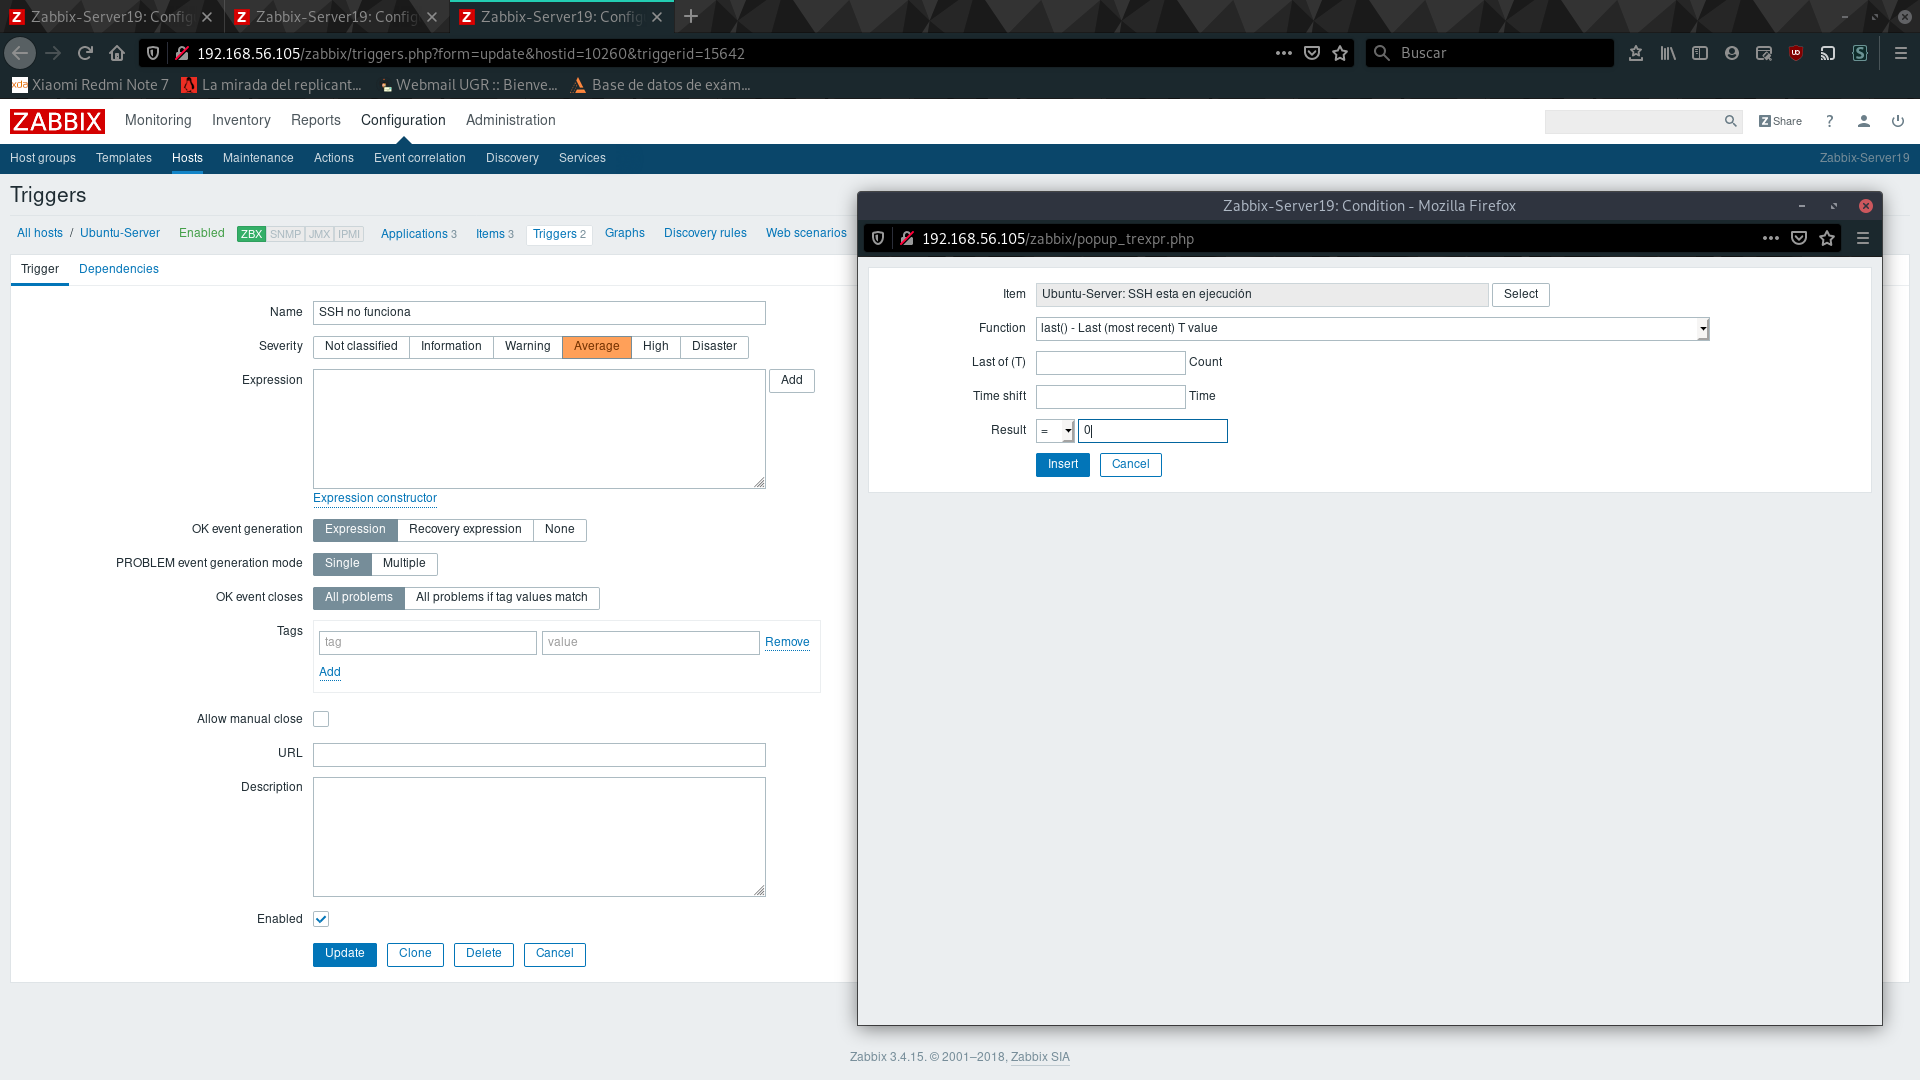
\includegraphics[scale=0.25]{ssh_trigger.png}
\end{center}


De esta forma, si paramos el servicio sshd, zabbix nos avisará:

\begin{center}
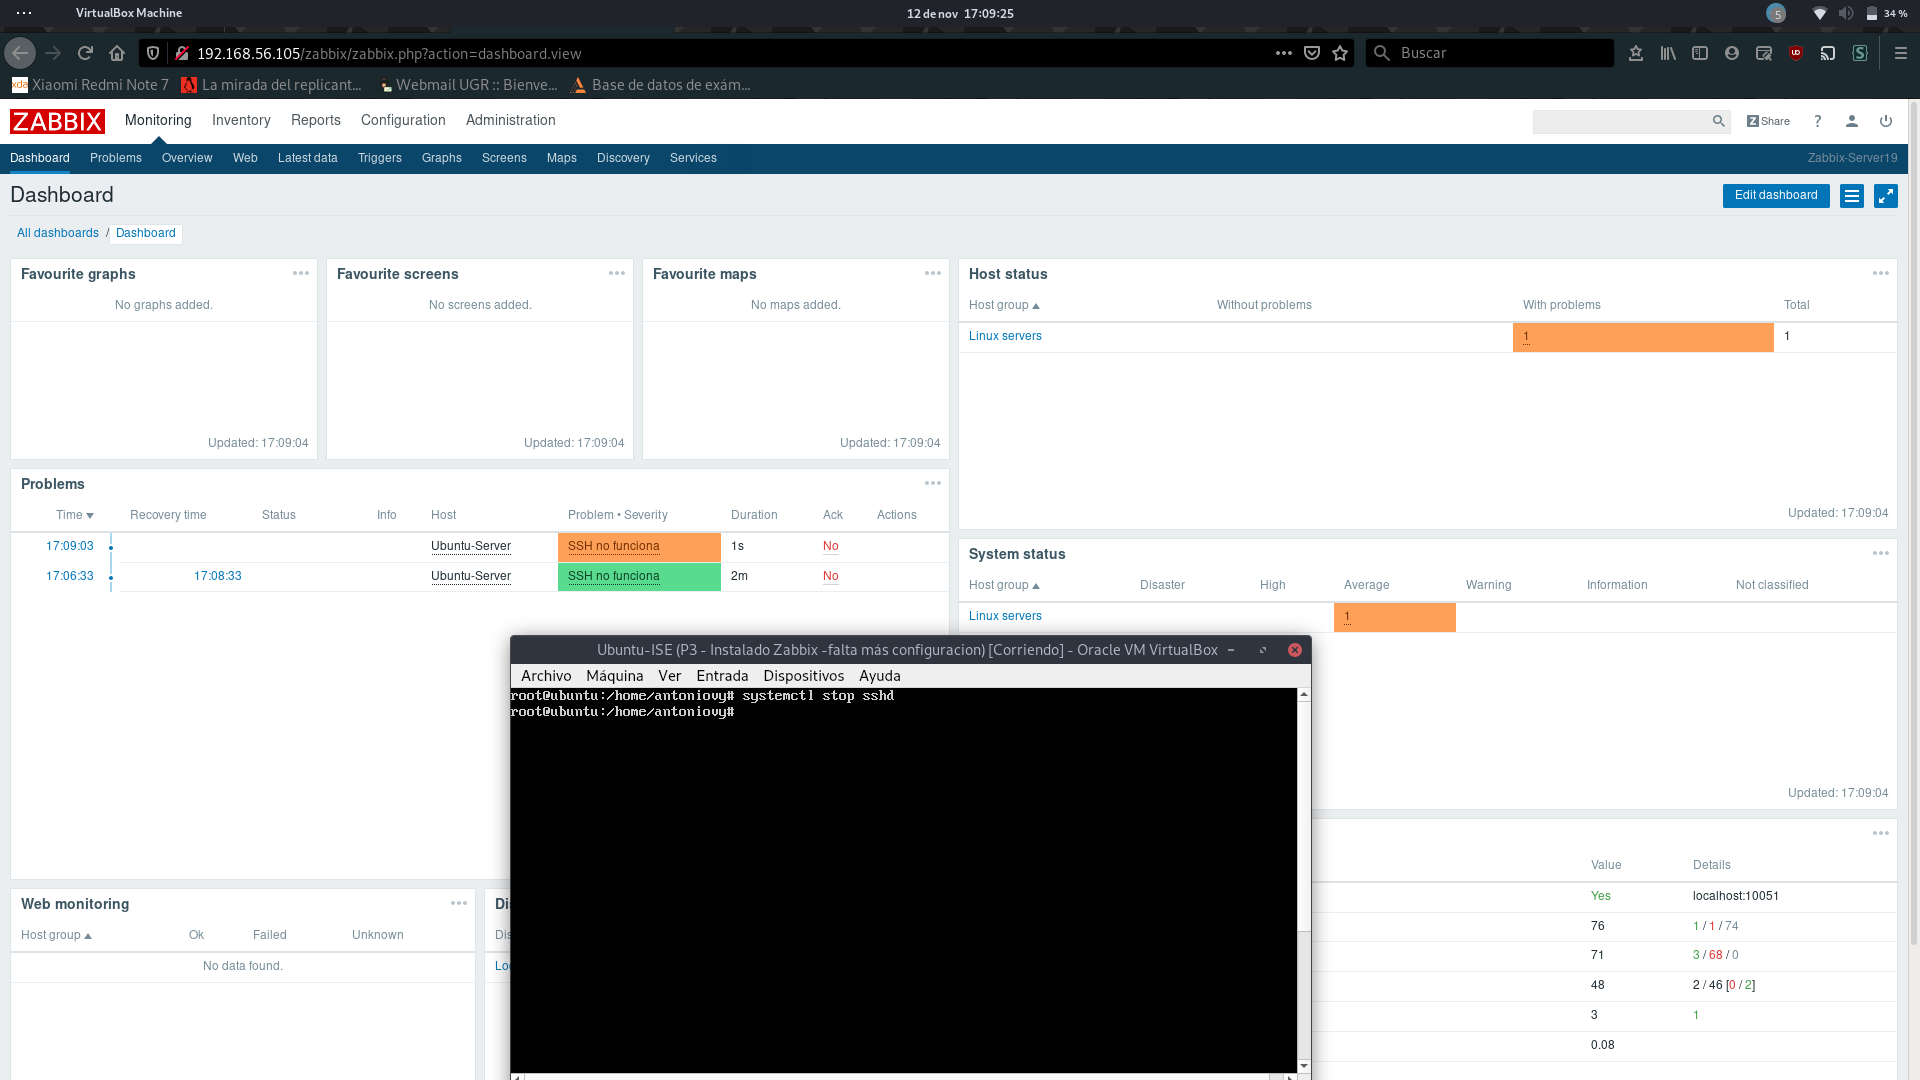
\includegraphics[scale=0.25]{ssh_stop.png}
\end{center}


Vemos también como hay un problema resuelto, esto se debe a que primero realicé una prueba parando sshd, al volver a iniciar el sshd Zabbix nos avisa que el problema ha sido resuelto.


\section{Conclusiones}

Como conclusión, vemos que Zabbix es un programa potente y versátil que permite monitorizar servidores de forma bastante sencilla, y además con una buena documentación y manuales.

Los pocos problemas que hemos encontrado (manejo de SELinux) le hemos podido encontrar  rápidamente solución gracias a la comunidad de Zabbix y sus foros, los cuales son bastante útiles y con bastante actividad entre usuarios.

Aunque nosotros hemos configurado Zabbix de una forma simple la complejidad de este software puede llegar a ser alta debido a la gran cantidad de opciones que ofrece, haciendo de este un buen servicio tanto para pequeños servidores como para sistemas más complejos.

\newpage

\begin{thebibliography}{9}

\bibitem{zabbix_man}
Manual Zabbix \url{https://www.zabbix.com/documentation/3.4/manual}

\bibitem{zabbix_apendice_BD}
Crear BD para Zabbix \url{https://www.zabbix.com/documentation/3.4/manual/appendix/install/db_scripts#mysql}

\bibitem{zabbix_quickstart}
Zabbix quickstart \url{https://www.zabbix.com/documentation/3.4/manual/quickstart/login}

\bibitem{zabbixSElinux}
Configurar Zabbix con SELinux  \url{https://www.zabbix.com/forum/zabbix-help/367261-selinux-and-zabbix}

\bibitem{audit2allow_man}
Manual audit2allow \url{https://linux.die.net/man/1/audit2allow}

\end{thebibliography}


\end{document}
